\documentclass[1p]{elsarticle_modified}
%\bibliographystyle{elsarticle-num}

%\usepackage[colorlinks]{hyperref}
%\usepackage{abbrmath_seonhwa} %\Abb, \Ascr, \Acal ,\Abf, \Afrak
\usepackage{amsfonts}
\usepackage{amssymb}
\usepackage{amsmath}
\usepackage{amsthm}
\usepackage{scalefnt}
\usepackage{amsbsy}
\usepackage{kotex}
\usepackage{caption}
\usepackage{subfig}
\usepackage{color}
\usepackage{graphicx}
\usepackage{xcolor} %% white, black, red, green, blue, cyan, magenta, yellow
\usepackage{float}
\usepackage{setspace}
\usepackage{hyperref}

\usepackage{tikz}
\usetikzlibrary{arrows}

\usepackage{multirow}
\usepackage{array} % fixed length table
\usepackage{hhline}

%%%%%%%%%%%%%%%%%%%%%
\makeatletter
\renewcommand*\env@matrix[1][\arraystretch]{%
	\edef\arraystretch{#1}%
	\hskip -\arraycolsep
	\let\@ifnextchar\new@ifnextchar
	\array{*\c@MaxMatrixCols c}}
\makeatother %https://tex.stackexchange.com/questions/14071/how-can-i-increase-the-line-spacing-in-a-matrix
%%%%%%%%%%%%%%%

\usepackage[normalem]{ulem}

\newcommand{\msout}[1]{\ifmmode\text{\sout{\ensuremath{#1}}}\else\sout{#1}\fi}
%SOURCE: \msout is \stkout macro in https://tex.stackexchange.com/questions/20609/strikeout-in-math-mode

\newcommand{\cancel}[1]{
	\ifmmode
	{\color{red}\msout{#1}}
	\else
	{\color{red}\sout{#1}}
	\fi
}

\newcommand{\add}[1]{
	{\color{blue}\uwave{#1}}
}

\newcommand{\replace}[2]{
	\ifmmode
	{\color{red}\msout{#1}}{\color{blue}\uwave{#2}}
	\else
	{\color{red}\sout{#1}}{\color{blue}\uwave{#2}}
	\fi
}

\newcommand{\Sol}{\mathcal{S}} %segment
\newcommand{\D}{D} %diagram
\newcommand{\A}{\mathcal{A}} %arc


%%%%%%%%%%%%%%%%%%%%%%%%%%%%%5 test

\def\sl{\operatorname{\textup{SL}}(2,\Cbb)}
\def\psl{\operatorname{\textup{PSL}}(2,\Cbb)}
\def\quan{\mkern 1mu \triangleright \mkern 1mu}

\theoremstyle{definition}
\newtheorem{thm}{Theorem}[section]
\newtheorem{prop}[thm]{Proposition}
\newtheorem{lem}[thm]{Lemma}
\newtheorem{ques}[thm]{Question}
\newtheorem{cor}[thm]{Corollary}
\newtheorem{defn}[thm]{Definition}
\newtheorem{exam}[thm]{Example}
\newtheorem{rmk}[thm]{Remark}
\newtheorem{alg}[thm]{Algorithm}

\newcommand{\I}{\sqrt{-1}}
\begin{document}

%\begin{frontmatter}
%
%\title{Boundary parabolic representations of knots up to 8 crossings}
%
%%% Group authors per affiliation:
%\author{Yunhi Cho} 
%\address{Department of Mathematics, University of Seoul, Seoul, Korea}
%\ead{yhcho@uos.ac.kr}
%
%
%\author{Seonhwa Kim} %\fnref{s_kim}}
%\address{Center for Geometry and Physics, Institute for Basic Science, Pohang, 37673, Korea}
%\ead{ryeona17@ibs.re.kr}
%
%\author{Hyuk Kim}
%\address{Department of Mathematical Sciences, Seoul National University, Seoul 08826, Korea}
%\ead{hyukkim@snu.ac.kr}
%
%\author{Seokbeom Yoon}
%\address{Department of Mathematical Sciences, Seoul National University, Seoul, 08826,  Korea}
%\ead{sbyoon15@snu.ac.kr}
%
%\begin{abstract}
%We find all boundary parabolic representation of knots up to 8 crossings.
%
%\end{abstract}
%\begin{keyword}
%    \MSC[2010] 57M25 
%\end{keyword}
%
%\end{frontmatter}

%\linenumbers
%\tableofcontents
%
\newcommand\colored[1]{\textcolor{white}{\rule[-0.35ex]{0.8em}{1.4ex}}\kern-0.8em\color{red} #1}%
%\newcommand\colored[1]{\textcolor{white}{ #1}\kern-2.17ex	\textcolor{white}{ #1}\kern-1.81ex	\textcolor{white}{ #1}\kern-2.15ex\color{red}#1	}

{\Large $\underline{12n_{0221}~(K12n_{0221})}$}

\setlength{\tabcolsep}{10pt}
\renewcommand{\arraystretch}{1.6}
\vspace{1cm}\begin{tabular}{m{100pt}>{\centering\arraybackslash}m{274pt}}
\multirow{5}{120pt}{
	\centering
	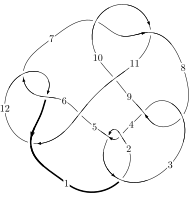
\includegraphics[width=112pt]{../../../GIT/diagram.site/Diagrams/png/2310_12n_0221.png}\\
\ \ \ A knot diagram\footnotemark}&
\allowdisplaybreaks
\textbf{Linearized knot diagam} \\
\cline{2-2}
 &
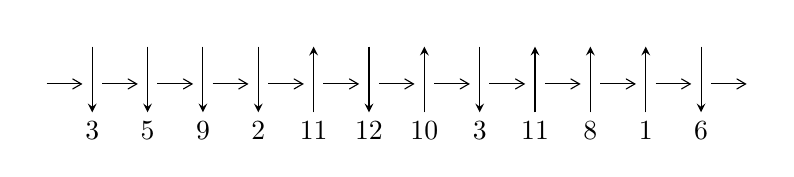
\begin{tikzpicture}[x=20pt, y=17pt]
	% nodes
	\node (C0) at (0, 0) {};
	\node (C1) at (1, 0) {};
	\node (C1U) at (1, +1) {};
	\node (C1D) at (1, -1) {3};

	\node (C2) at (2, 0) {};
	\node (C2U) at (2, +1) {};
	\node (C2D) at (2, -1) {5};

	\node (C3) at (3, 0) {};
	\node (C3U) at (3, +1) {};
	\node (C3D) at (3, -1) {9};

	\node (C4) at (4, 0) {};
	\node (C4U) at (4, +1) {};
	\node (C4D) at (4, -1) {2};

	\node (C5) at (5, 0) {};
	\node (C5U) at (5, +1) {};
	\node (C5D) at (5, -1) {11};

	\node (C6) at (6, 0) {};
	\node (C6U) at (6, +1) {};
	\node (C6D) at (6, -1) {12};

	\node (C7) at (7, 0) {};
	\node (C7U) at (7, +1) {};
	\node (C7D) at (7, -1) {10};

	\node (C8) at (8, 0) {};
	\node (C8U) at (8, +1) {};
	\node (C8D) at (8, -1) {3};

	\node (C9) at (9, 0) {};
	\node (C9U) at (9, +1) {};
	\node (C9D) at (9, -1) {11};

	\node (C10) at (10, 0) {};
	\node (C10U) at (10, +1) {};
	\node (C10D) at (10, -1) {8};

	\node (C11) at (11, 0) {};
	\node (C11U) at (11, +1) {};
	\node (C11D) at (11, -1) {1};

	\node (C12) at (12, 0) {};
	\node (C12U) at (12, +1) {};
	\node (C12D) at (12, -1) {6};
	\node (C13) at (13, 0) {};

	% arrows
	\draw[->,>={angle 60}]
	(C0) edge (C1) (C1) edge (C2) (C2) edge (C3) (C3) edge (C4) (C4) edge (C5) (C5) edge (C6) (C6) edge (C7) (C7) edge (C8) (C8) edge (C9) (C9) edge (C10) (C10) edge (C11) (C11) edge (C12) (C12) edge (C13) ;	\draw[->,>=stealth]
	(C1U) edge (C1D) (C2U) edge (C2D) (C3U) edge (C3D) (C4U) edge (C4D) (C5D) edge (C5U) (C6U) edge (C6D) (C7D) edge (C7U) (C8U) edge (C8D) (C9D) edge (C9U) (C10D) edge (C10U) (C11D) edge (C11U) (C12U) edge (C12D) ;
	\end{tikzpicture} \\
\hhline{~~} \\& 
\textbf{Solving Sequence} \\ \cline{2-2} 
 &
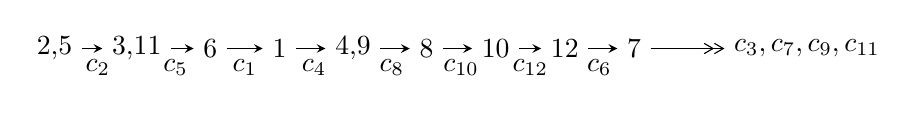
\begin{tikzpicture}[x=25pt, y=7pt]
	% node
	\node (A0) at (-1/8, 0) {2,5};
	\node (A1) at (17/16, 0) {3,11};
	\node (A2) at (17/8, 0) {6};
	\node (A3) at (25/8, 0) {1};
	\node (A4) at (67/16, 0) {4,9};
	\node (A5) at (21/4, 0) {8};
	\node (A6) at (25/4, 0) {10};
	\node (A7) at (29/4, 0) {12};
	\node (A8) at (33/4, 0) {7};
	\node (C1) at (1/2, -1) {$c_{2}$};
	\node (C2) at (13/8, -1) {$c_{5}$};
	\node (C3) at (21/8, -1) {$c_{1}$};
	\node (C4) at (29/8, -1) {$c_{4}$};
	\node (C5) at (19/4, -1) {$c_{8}$};
	\node (C6) at (23/4, -1) {$c_{10}$};
	\node (C7) at (27/4, -1) {$c_{12}$};
	\node (C8) at (31/4, -1) {$c_{6}$};
	\node (A9) at (43/4, 0) {$c_{3},c_{7},c_{9},c_{11}$};

	% edge
	\draw[->,>=stealth]	
	(A0) edge (A1) (A1) edge (A2) (A2) edge (A3) (A3) edge (A4) (A4) edge (A5) (A5) edge (A6) (A6) edge (A7) (A7) edge (A8) ;
	\draw[->>,>={angle 60}]	
	(A8) edge (A9);
\end{tikzpicture} \\ 

\end{tabular} \\

\footnotetext{
The image of knot diagram is generated by the software ``\textbf{Draw programme}" developed by Andrew Bartholomew(\url{http://www.layer8.co.uk/maths/draw/index.htm\#Running-draw}), where we modified some parts for our purpose(\url{https://github.com/CATsTAILs/LinksPainter}).
}\phantom \\ \newline 
\centering \textbf{Ideals for irreducible components\footnotemark of $X_{\text{par}}$} 
 
\begin{align*}
I^u_{1}&=\langle 
2258808925 u^{16}+15860359921 u^{15}+\cdots+96479313856 d-115431185160,\\
\phantom{I^u_{1}}&\phantom{= \langle  }154139657205 u^{16}+1193150529938 u^{15}+\cdots+2508462160256 c-2116899433348,\\
\phantom{I^u_{1}}&\phantom{= \langle  }4410667 u^{16}+32637095 u^{15}+\cdots+83243584 b-126220048,\\
\phantom{I^u_{1}}&\phantom{= \langle  }7888753 u^{16}+58699357 u^{15}+\cdots+83243584 a-107418368,\;u^{17}+8 u^{16}+\cdots-8 u-16\rangle \\
I^u_{2}&=\langle 
d- a,\;c- a,\;b- a,\;a^2- a+1,\;u-1\rangle \\
I^u_{3}&=\langle 
d+1,\;c,\;b-1,\;a-1,\;u-1\rangle \\
I^u_{4}&=\langle 
d a- c a+1,\;c^2- c+1,\;b- a,\;u-1\rangle \\
\\
I^v_{1}&=\langle 
c,\;d- a-1,\;b,\;a^2+a+1,\;v-1\rangle \\
\end{align*}
\raggedright * 4 irreducible components of $\dim_{\mathbb{C}}=0$, with total 22 representations.\\
\raggedright * 1 irreducible components of $\dim_{\mathbb{C}}=1$ \\
\footnotetext{All coefficients of polynomials are rational numbers. But the coefficients are sometimes approximated in decimal forms when there is not enough margin.}
\newpage
\renewcommand{\arraystretch}{1}
\centering \section*{I. $I^u_{1}= \langle 2.26\times10^{9} u^{16}+1.59\times10^{10} u^{15}+\cdots+9.65\times10^{10} d-1.15\times10^{11},\;1.54\times10^{11} u^{16}+1.19\times10^{12} u^{15}+\cdots+2.51\times10^{12} c-2.12\times10^{12},\;4.41\times10^{6} u^{16}+3.26\times10^{7} u^{15}+\cdots+8.32\times10^{7} b-1.26\times10^{8},\;7.89\times10^{6} u^{16}+5.87\times10^{7} u^{15}+\cdots+8.32\times10^{7} a-1.07\times10^{8},\;u^{17}+8 u^{16}+\cdots-8 u-16 \rangle$}
\flushleft \textbf{(i) Arc colorings}\\
\begin{tabular}{m{7pt} m{180pt} m{7pt} m{180pt} }
\flushright $a_{2}=$&$\begin{pmatrix}1\\0\end{pmatrix}$ \\
\flushright $a_{5}=$&$\begin{pmatrix}0\\u\end{pmatrix}$ \\
\flushright $a_{3}=$&$\begin{pmatrix}1\\u^2\end{pmatrix}$ \\
\flushright $a_{11}=$&$\begin{pmatrix}-0.0614479 u^{16}-0.475650 u^{15}+\cdots-2.87951 u+0.843903\\-0.0234124 u^{16}-0.164391 u^{15}+\cdots+0.757508 u+1.19643\end{pmatrix}$ \\
\flushright $a_{6}=$&$\begin{pmatrix}0.0269638 u^{16}+0.213054 u^{15}+\cdots+1.26938 u+0.117878\\-0.00435471 u^{16}-0.0521688 u^{15}+\cdots+0.124403 u-0.745012\end{pmatrix}$ \\
\flushright $a_{1}=$&$\begin{pmatrix}- u^2+1\\- u^4\end{pmatrix}$ \\
\flushright $a_{4}=$&$\begin{pmatrix}u\\u\end{pmatrix}$ \\
\flushright $a_{9}=$&$\begin{pmatrix}-0.0947671 u^{16}-0.705152 u^{15}+\cdots+0.385893 u+1.29041\\-0.0529851 u^{16}-0.392067 u^{15}+\cdots-0.532273 u+1.51627\end{pmatrix}$ \\
\flushright $a_{8}=$&$\begin{pmatrix}-0.115939 u^{16}-0.867332 u^{15}+\cdots+0.946013 u+1.95892\\-0.0618930 u^{16}-0.460152 u^{15}+\cdots-0.813462 u+1.63140\end{pmatrix}$ \\
\flushright $a_{10}=$&$\begin{pmatrix}-0.118012 u^{16}-0.895172 u^{15}+\cdots-0.266541 u+1.78486\\-0.0519178 u^{16}-0.373867 u^{15}+\cdots+0.197985 u+1.94957\end{pmatrix}$ \\
\flushright $a_{12}=$&$\begin{pmatrix}-0.0656989 u^{16}-0.494197 u^{15}+\cdots-2.08468 u+1.58103\\-0.0178046 u^{16}-0.118986 u^{15}+\cdots+0.894693 u+1.10503\end{pmatrix}$ \\
\flushright $a_{7}=$&$\begin{pmatrix}0.0678023 u^{16}+0.515689 u^{15}+\cdots+1.99680 u-0.449277\\0.0201677 u^{16}+0.140474 u^{15}+\cdots+0.214188 u-1.03624\end{pmatrix}$\\&\end{tabular}
\flushleft \textbf{(ii) Obstruction class $= -1$}\\~\\
\flushleft \textbf{(iii) Cusp Shapes $= -\frac{3288027181}{156778885016} u^{16}-\frac{220303787499}{627115540064} u^{15}+\cdots-\frac{1274298730399}{156778885016} u-\frac{92162275708}{19597360627}$}\\~\\
\newpage\renewcommand{\arraystretch}{1}
\flushleft \textbf{(iv) u-Polynomials at the component}\newline \\
\begin{tabular}{m{50pt}|m{274pt}}
Crossings & \hspace{64pt}u-Polynomials at each crossing \\
\hline $$\begin{aligned}c_{1}\end{aligned}$$&$\begin{aligned}
&u^{17}-6 u^{16}+\cdots+32 u+256
\end{aligned}$\\
\hline $$\begin{aligned}c_{2},c_{4}\end{aligned}$$&$\begin{aligned}
&u^{17}-8 u^{16}+\cdots-8 u+16
\end{aligned}$\\
\hline $$\begin{aligned}c_{3},c_{8}\end{aligned}$$&$\begin{aligned}
&u^{17}+u^{16}+\cdots-1024 u+512
\end{aligned}$\\
\hline $$\begin{aligned}c_{5}\end{aligned}$$&$\begin{aligned}
&u^{17}+14 u^{16}+\cdots+6768 u+2592
\end{aligned}$\\
\hline $$\begin{aligned}c_{6},c_{12}\end{aligned}$$&$\begin{aligned}
&u^{17}-5 u^{16}+\cdots-11 u^2+4
\end{aligned}$\\
\hline $$\begin{aligned}c_{7},c_{10}\end{aligned}$$&$\begin{aligned}
&u^{17}+8 u^{16}+\cdots-8 u+16
\end{aligned}$\\
\hline $$\begin{aligned}c_{9}\end{aligned}$$&$\begin{aligned}
&u^{17}-34 u^{16}+\cdots+6176 u-256
\end{aligned}$\\
\hline $$\begin{aligned}c_{11}\end{aligned}$$&$\begin{aligned}
&u^{17}-15 u^{16}+\cdots+88 u+16
\end{aligned}$\\
\hline
\end{tabular}\\~\\
\newpage\renewcommand{\arraystretch}{1}
\flushleft \textbf{(v) Riley Polynomials at the component}\newline \\
\begin{tabular}{m{50pt}|m{274pt}}
Crossings & \hspace{64pt}Riley Polynomials at each crossing \\
\hline $$\begin{aligned}c_{1}\end{aligned}$$&$\begin{aligned}
&y^{17}+66 y^{16}+\cdots+2613760 y-65536
\end{aligned}$\\
\hline $$\begin{aligned}c_{2},c_{4}\end{aligned}$$&$\begin{aligned}
&y^{17}+6 y^{16}+\cdots+32 y-256
\end{aligned}$\\
\hline $$\begin{aligned}c_{3},c_{8}\end{aligned}$$&$\begin{aligned}
&y^{17}+81 y^{16}+\cdots-524288 y-262144
\end{aligned}$\\
\hline $$\begin{aligned}c_{5}\end{aligned}$$&$\begin{aligned}
&y^{17}-66 y^{16}+\cdots+36764928 y-6718464
\end{aligned}$\\
\hline $$\begin{aligned}c_{6},c_{12}\end{aligned}$$&$\begin{aligned}
&y^{17}+15 y^{16}+\cdots+88 y-16
\end{aligned}$\\
\hline $$\begin{aligned}c_{7},c_{10}\end{aligned}$$&$\begin{aligned}
&y^{17}-34 y^{16}+\cdots+6176 y-256
\end{aligned}$\\
\hline $$\begin{aligned}c_{9}\end{aligned}$$&$\begin{aligned}
&y^{17}-94 y^{16}+\cdots+7397888 y-65536
\end{aligned}$\\
\hline $$\begin{aligned}c_{11}\end{aligned}$$&$\begin{aligned}
&y^{17}-21 y^{16}+\cdots+36640 y-256
\end{aligned}$\\
\hline
\end{tabular}\\~\\
\newpage\flushleft \textbf{(vi) Complex Volumes and Cusp Shapes}
$$\begin{array}{c|c|c}  
\text{Solutions to }I^u_{1}& \I (\text{vol} + \sqrt{-1}CS) & \text{Cusp shape}\\
 \hline 
\begin{aligned}
u &= \phantom{-}0.789321\phantom{ +0.000000I} \\
a &= \phantom{-}0.386224\phantom{ +0.000000I} \\
b &= -0.304855\phantom{ +0.000000I} \\
c &= \phantom{-}0.374974\phantom{ +0.000000I} \\
d &= -0.586930\phantom{ +0.000000I}\end{aligned}
 & -1.13318\phantom{ +0.000000I} & -9.61860\phantom{ +0.000000I} \\ \hline\begin{aligned}
u &= \phantom{-}1.281020 + 0.078323 I \\
a &= \phantom{-}0.027802 - 0.314358 I \\
b &= -0.060236 + 0.400521 I \\
c &= \phantom{-}0.519378 - 0.243814 I \\
d &= \phantom{-}0.992769 + 0.281518 I\end{aligned}
 & -0.72956 - 1.37071 I & -0.698150 + 0.213889 I \\ \hline\begin{aligned}
u &= \phantom{-}1.281020 - 0.078323 I \\
a &= \phantom{-}0.027802 + 0.314358 I \\
b &= -0.060236 - 0.400521 I \\
c &= \phantom{-}0.519378 + 0.243814 I \\
d &= \phantom{-}0.992769 - 0.281518 I\end{aligned}
 & -0.72956 + 1.37071 I & -0.698150 - 0.213889 I \\ \hline\begin{aligned}
u &= -0.709544 + 0.075286 I \\
a &= \phantom{-}0.27087 + 2.81412 I \\
b &= \phantom{-}0.40406 + 1.97635 I \\
c &= \phantom{-}0.41875 + 1.62653 I \\
d &= \phantom{-}0.386110 + 1.184900 I\end{aligned}
 & -0.79868 + 2.33972 I & \phantom{-}0.33078 - 5.26516 I \\ \hline\begin{aligned}
u &= -0.709544 - 0.075286 I \\
a &= \phantom{-}0.27087 - 2.81412 I \\
b &= \phantom{-}0.40406 - 1.97635 I \\
c &= \phantom{-}0.41875 - 1.62653 I \\
d &= \phantom{-}0.386110 - 1.184900 I\end{aligned}
 & -0.79868 - 2.33972 I & \phantom{-}0.33078 + 5.26516 I \\ \hline\begin{aligned}
u &= \phantom{-}0.491842 + 0.197993 I \\
a &= -0.746901 + 0.354453 I \\
b &= \phantom{-}0.437536 - 0.026454 I \\
c &= -0.68906 + 1.41559 I \\
d &= \phantom{-}1.212590 - 0.601554 I\end{aligned}
 & \phantom{-}0.77904 - 2.74622 I & -2.48507 + 7.16740 I\\
 \hline 
 \end{array}$$\newpage$$\begin{array}{c|c|c}  
\text{Solutions to }I^u_{1}& \I (\text{vol} + \sqrt{-1}CS) & \text{Cusp shape}\\
 \hline 
\begin{aligned}
u &= \phantom{-}0.491842 - 0.197993 I \\
a &= -0.746901 - 0.354453 I \\
b &= \phantom{-}0.437536 + 0.026454 I \\
c &= -0.68906 - 1.41559 I \\
d &= \phantom{-}1.212590 + 0.601554 I\end{aligned}
 & \phantom{-}0.77904 + 2.74622 I & -2.48507 - 7.16740 I \\ \hline\begin{aligned}
u &= -0.118015 + 0.350813 I \\
a &= -0.50791 + 1.75422 I \\
b &= \phantom{-}0.555461 + 0.385207 I \\
c &= \phantom{-}1.154330 + 0.052946 I \\
d &= \phantom{-}0.083184 + 0.147223 I\end{aligned}
 & \phantom{-}1.75773 + 0.71028 I & \phantom{-}3.71531 + 0.02644 I \\ \hline\begin{aligned}
u &= -0.118015 - 0.350813 I \\
a &= -0.50791 - 1.75422 I \\
b &= \phantom{-}0.555461 - 0.385207 I \\
c &= \phantom{-}1.154330 - 0.052946 I \\
d &= \phantom{-}0.083184 - 0.147223 I\end{aligned}
 & \phantom{-}1.75773 - 0.71028 I & \phantom{-}3.71531 - 0.02644 I \\ \hline\begin{aligned}
u &= -1.65818 + 0.90820 I \\
a &= \phantom{-}0.976512 + 0.609189 I \\
b &= \phantom{-}2.17250 + 0.12328 I \\
c &= -0.94081 - 1.33349 I \\
d &= -5.94499 - 2.01193 I\end{aligned}
 & \phantom{-}18.4182 + 12.9335 I & -1.01650 - 5.27491 I \\ \hline\begin{aligned}
u &= -1.65818 - 0.90820 I \\
a &= \phantom{-}0.976512 - 0.609189 I \\
b &= \phantom{-}2.17250 - 0.12328 I \\
c &= -0.94081 + 1.33349 I \\
d &= -5.94499 + 2.01193 I\end{aligned}
 & \phantom{-}18.4182 - 12.9335 I & -1.01650 + 5.27491 I \\ \hline\begin{aligned}
u &= -1.62328 + 1.28695 I \\
a &= -0.780321 - 0.614432 I \\
b &= -2.05742 + 0.00684 I \\
c &= \phantom{-}0.67125 + 1.78783 I \\
d &= \phantom{-}8.16028 + 1.30179 I\end{aligned}
 & \phantom{-}15.3110 + 5.6503 I & -2.10303 - 1.68119 I\\
 \hline 
 \end{array}$$\newpage$$\begin{array}{c|c|c}  
\text{Solutions to }I^u_{1}& \I (\text{vol} + \sqrt{-1}CS) & \text{Cusp shape}\\
 \hline 
\begin{aligned}
u &= -1.62328 - 1.28695 I \\
a &= -0.780321 + 0.614432 I \\
b &= -2.05742 - 0.00684 I \\
c &= \phantom{-}0.67125 - 1.78783 I \\
d &= \phantom{-}8.16028 - 1.30179 I\end{aligned}
 & \phantom{-}15.3110 - 5.6503 I & -2.10303 + 1.68119 I \\ \hline\begin{aligned}
u &= -0.77580 + 2.21598 I \\
a &= -0.394911 - 0.622157 I \\
b &= -1.68506 + 0.39245 I \\
c &= -1.69156 - 0.56408 I \\
d &= \phantom{-}4.42924 + 7.49395 I\end{aligned}
 & \phantom{-}9.63429 + 3.26152 I & \phantom{-}0.10201 - 1.44169 I \\ \hline\begin{aligned}
u &= -0.77580 - 2.21598 I \\
a &= -0.394911 + 0.622157 I \\
b &= -1.68506 - 0.39245 I \\
c &= -1.69156 + 0.56408 I \\
d &= \phantom{-}4.42924 - 7.49395 I\end{aligned}
 & \phantom{-}9.63429 - 3.26152 I & \phantom{-}0.10201 + 1.44169 I \\ \hline\begin{aligned}
u &= -1.28271 + 2.40373 I \\
a &= \phantom{-}0.461749 + 0.538038 I \\
b &= \phantom{-}1.88559 - 0.41977 I \\
c &= -0.25477 - 2.11813 I \\
d &= -12.0257 + 7.8857 I\end{aligned}
 & -17.4865 - 1.7702 I & \phantom{-0.000000 -}     -6
0. 10   + 0.657690 I \\ \hline\begin{aligned}
u &= -1.28271 - 2.40373 I \\
a &= \phantom{-}0.461749 - 0.538038 I \\
b &= \phantom{-}1.88559 + 0.41977 I \\
c &= -0.25477 + 2.11813 I \\
d &= -12.0257 - 7.8857 I\end{aligned}
 & -17.4865 + 1.7702 I & \phantom{-0.000000 }      -6
0. 10   - 0.657690 I\\
 \hline 
 \end{array}$$\newpage\newpage\renewcommand{\arraystretch}{1}
\centering \section*{II. $I^u_{2}= \langle d- a,\;c- a,\;b- a,\;a^2- a+1,\;u-1 \rangle$}
\flushleft \textbf{(i) Arc colorings}\\
\begin{tabular}{m{7pt} m{180pt} m{7pt} m{180pt} }
\flushright $a_{2}=$&$\begin{pmatrix}1\\0\end{pmatrix}$ \\
\flushright $a_{5}=$&$\begin{pmatrix}0\\1\end{pmatrix}$ \\
\flushright $a_{3}=$&$\begin{pmatrix}1\\1\end{pmatrix}$ \\
\flushright $a_{11}=$&$\begin{pmatrix}a\\a\end{pmatrix}$ \\
\flushright $a_{6}=$&$\begin{pmatrix}a-1\\a\end{pmatrix}$ \\
\flushright $a_{1}=$&$\begin{pmatrix}0\\-1\end{pmatrix}$ \\
\flushright $a_{4}=$&$\begin{pmatrix}1\\1\end{pmatrix}$ \\
\flushright $a_{9}=$&$\begin{pmatrix}a\\a\end{pmatrix}$ \\
\flushright $a_{8}=$&$\begin{pmatrix}a\\a\end{pmatrix}$ \\
\flushright $a_{10}=$&$\begin{pmatrix}a\\a\end{pmatrix}$ \\
\flushright $a_{12}=$&$\begin{pmatrix}a\\0\end{pmatrix}$ \\
\flushright $a_{7}=$&$\begin{pmatrix}a\\a\end{pmatrix}$\\&\end{tabular}
\flushleft \textbf{(ii) Obstruction class $= 1$}\\~\\
\flushleft \textbf{(iii) Cusp Shapes $= -4 a-7$}\\~\\
\newpage\renewcommand{\arraystretch}{1}
\flushleft \textbf{(iv) u-Polynomials at the component}\newline \\
\begin{tabular}{m{50pt}|m{274pt}}
Crossings & \hspace{64pt}u-Polynomials at each crossing \\
\hline $$\begin{aligned}c_{1},c_{2}\end{aligned}$$&$\begin{aligned}
&(u-1)^2
\end{aligned}$\\
\hline $$\begin{aligned}c_{3},c_{7},c_{8}\\c_{9},c_{10}\end{aligned}$$&$\begin{aligned}
&u^2
\end{aligned}$\\
\hline $$\begin{aligned}c_{4}\end{aligned}$$&$\begin{aligned}
&(u+1)^2
\end{aligned}$\\
\hline $$\begin{aligned}c_{5},c_{11},c_{12}\end{aligned}$$&$\begin{aligned}
&u^2+u+1
\end{aligned}$\\
\hline $$\begin{aligned}c_{6}\end{aligned}$$&$\begin{aligned}
&u^2- u+1
\end{aligned}$\\
\hline
\end{tabular}\\~\\
\newpage\renewcommand{\arraystretch}{1}
\flushleft \textbf{(v) Riley Polynomials at the component}\newline \\
\begin{tabular}{m{50pt}|m{274pt}}
Crossings & \hspace{64pt}Riley Polynomials at each crossing \\
\hline $$\begin{aligned}c_{1},c_{2},c_{4}\end{aligned}$$&$\begin{aligned}
&(y-1)^2
\end{aligned}$\\
\hline $$\begin{aligned}c_{3},c_{7},c_{8}\\c_{9},c_{10}\end{aligned}$$&$\begin{aligned}
&y^2
\end{aligned}$\\
\hline $$\begin{aligned}c_{5},c_{6},c_{11}\\c_{12}\end{aligned}$$&$\begin{aligned}
&y^2+y+1
\end{aligned}$\\
\hline
\end{tabular}\\~\\
\newpage\flushleft \textbf{(vi) Complex Volumes and Cusp Shapes}
$$\begin{array}{c|c|c}  
\text{Solutions to }I^u_{2}& \I (\text{vol} + \sqrt{-1}CS) & \text{Cusp shape}\\
 \hline 
\begin{aligned}
u &= \phantom{-}1.00000\phantom{ +0.000000I} \\
a &= \phantom{-}0.500000 + 0.866025 I \\
b &= \phantom{-}0.500000 + 0.866025 I \\
c &= \phantom{-}0.500000 + 0.866025 I \\
d &= \phantom{-}0.500000 + 0.866025 I\end{aligned}
 & -1.64493 + 2.02988 I & -9.00000 - 3.46410 I \\ \hline\begin{aligned}
u &= \phantom{-}1.00000\phantom{ +0.000000I} \\
a &= \phantom{-}0.500000 - 0.866025 I \\
b &= \phantom{-}0.500000 - 0.866025 I \\
c &= \phantom{-}0.500000 - 0.866025 I \\
d &= \phantom{-}0.500000 - 0.866025 I\end{aligned}
 & -1.64493 - 2.02988 I & -9.00000 + 3.46410 I\\
 \hline 
 \end{array}$$\newpage\newpage\renewcommand{\arraystretch}{1}
\centering \section*{III. $I^u_{3}= \langle d+1,\;c,\;b-1,\;a-1,\;u-1 \rangle$}
\flushleft \textbf{(i) Arc colorings}\\
\begin{tabular}{m{7pt} m{180pt} m{7pt} m{180pt} }
\flushright $a_{2}=$&$\begin{pmatrix}1\\0\end{pmatrix}$ \\
\flushright $a_{5}=$&$\begin{pmatrix}0\\1\end{pmatrix}$ \\
\flushright $a_{3}=$&$\begin{pmatrix}1\\1\end{pmatrix}$ \\
\flushright $a_{11}=$&$\begin{pmatrix}0\\-1\end{pmatrix}$ \\
\flushright $a_{6}=$&$\begin{pmatrix}0\\1\end{pmatrix}$ \\
\flushright $a_{1}=$&$\begin{pmatrix}0\\-1\end{pmatrix}$ \\
\flushright $a_{4}=$&$\begin{pmatrix}1\\1\end{pmatrix}$ \\
\flushright $a_{9}=$&$\begin{pmatrix}1\\1\end{pmatrix}$ \\
\flushright $a_{8}=$&$\begin{pmatrix}1\\1\end{pmatrix}$ \\
\flushright $a_{10}=$&$\begin{pmatrix}1\\0\end{pmatrix}$ \\
\flushright $a_{12}=$&$\begin{pmatrix}0\\-1\end{pmatrix}$ \\
\flushright $a_{7}=$&$\begin{pmatrix}0\\1\end{pmatrix}$\\&\end{tabular}
\flushleft \textbf{(ii) Obstruction class $= 1$}\\~\\
\flushleft \textbf{(iii) Cusp Shapes $= 0$}\\~\\
\newpage\renewcommand{\arraystretch}{1}
\flushleft \textbf{(iv) u-Polynomials at the component}\newline \\
\begin{tabular}{m{50pt}|m{274pt}}
Crossings & \hspace{64pt}u-Polynomials at each crossing \\
\hline $$\begin{aligned}c_{1},c_{2},c_{10}\end{aligned}$$&$\begin{aligned}
&u-1
\end{aligned}$\\
\hline $$\begin{aligned}c_{3},c_{5},c_{6}\\c_{8},c_{11},c_{12}\end{aligned}$$&$\begin{aligned}
&u
\end{aligned}$\\
\hline $$\begin{aligned}c_{4},c_{7},c_{9}\end{aligned}$$&$\begin{aligned}
&u+1
\end{aligned}$\\
\hline
\end{tabular}\\~\\
\newpage\renewcommand{\arraystretch}{1}
\flushleft \textbf{(v) Riley Polynomials at the component}\newline \\
\begin{tabular}{m{50pt}|m{274pt}}
Crossings & \hspace{64pt}Riley Polynomials at each crossing \\
\hline $$\begin{aligned}c_{1},c_{2},c_{4}\\c_{7},c_{9},c_{10}\end{aligned}$$&$\begin{aligned}
&y-1
\end{aligned}$\\
\hline $$\begin{aligned}c_{3},c_{5},c_{6}\\c_{8},c_{11},c_{12}\end{aligned}$$&$\begin{aligned}
&y
\end{aligned}$\\
\hline
\end{tabular}\\~\\
\newpage\flushleft \textbf{(vi) Complex Volumes and Cusp Shapes}
$$\begin{array}{c|c|c}  
\text{Solutions to }I^u_{3}& \I (\text{vol} + \sqrt{-1}CS) & \text{Cusp shape}\\
 \hline 
\begin{aligned}
u &= \phantom{-}1.00000\phantom{ +0.000000I} \\
a &= \phantom{-}1.00000\phantom{ +0.000000I} \\
b &= \phantom{-}1.00000\phantom{ +0.000000I} \\
c &= \phantom{-0.000000 } 0 \\
d &= -1.00000\phantom{ +0.000000I}\end{aligned}
 & \phantom{-0.000000 } 0 & \phantom{-0.000000 } 0\\
 \hline 
 \end{array}$$\newpage\newpage\renewcommand{\arraystretch}{1}
\centering \section*{IV. $I^u_{4}= \langle d a- c a+1,\;c^2- c+1,\;b- a,\;u-1 \rangle$}
\flushleft \textbf{(i) Arc colorings}\\
\begin{tabular}{m{7pt} m{180pt} m{7pt} m{180pt} }
\flushright $a_{2}=$&$\begin{pmatrix}1\\0\end{pmatrix}$ \\
\flushright $a_{5}=$&$\begin{pmatrix}0\\1\end{pmatrix}$ \\
\flushright $a_{3}=$&$\begin{pmatrix}1\\1\end{pmatrix}$ \\
\flushright $a_{11}=$&$\begin{pmatrix}c\\d\end{pmatrix}$ \\
\flushright $a_{6}=$&$\begin{pmatrix}c-1\\d c+1\end{pmatrix}$ \\
\flushright $a_{1}=$&$\begin{pmatrix}0\\-1\end{pmatrix}$ \\
\flushright $a_{4}=$&$\begin{pmatrix}1\\1\end{pmatrix}$ \\
\flushright $a_{9}=$&$\begin{pmatrix}a\\a\end{pmatrix}$ \\
\flushright $a_{8}=$&$\begin{pmatrix}a\\a\end{pmatrix}$ \\
\flushright $a_{10}=$&$\begin{pmatrix}c+a\\d+a\end{pmatrix}$ \\
\flushright $a_{12}=$&$\begin{pmatrix}c\\d- c\end{pmatrix}$ \\
\flushright $a_{7}=$&$\begin{pmatrix}c\\d\end{pmatrix}$\\&\end{tabular}
\flushleft \textbf{(ii) Obstruction class $= -1$}\\~\\
\flushleft \textbf{(iii) Cusp Shapes $= d^2-2 d c+a^2-3 c-1$}\\~\\
\flushleft \textbf{(iv) u-Polynomials at the component} : It cannot be defined for a positive dimension component.\\~\\
\flushleft \textbf{(v) Riley Polynomials at the component} : It cannot be defined for a positive dimension component.\\~\\
\newpage\flushleft \textbf{(iv) Complex Volumes and Cusp Shapes}
$$\begin{array}{c|c|c} 
\text{Solution to }I^u_{4}& \I (\text{vol} + \sqrt{-1}CS) & \text{Cusp shape}\\
 \hline 
\begin{aligned}
u &= \cdots \\
a &= \cdots \\
b &= \cdots \\
c &= \cdots \\
d &= \cdots\end{aligned}
 & \phantom{-0.000000 } -2.02988 I & -0.06692 - 3.42770 I\\
 \hline 
 \end{array}
$$\newpage\renewcommand{\arraystretch}{1}
\centering \section*{V. $I^v_{1}= \langle c,\;d- a-1,\;b,\;a^2+a+1,\;v-1 \rangle$}
\flushleft \textbf{(i) Arc colorings}\\
\begin{tabular}{m{7pt} m{180pt} m{7pt} m{180pt} }
\flushright $a_{2}=$&$\begin{pmatrix}1\\0\end{pmatrix}$ \\
\flushright $a_{5}=$&$\begin{pmatrix}1\\0\end{pmatrix}$ \\
\flushright $a_{3}=$&$\begin{pmatrix}1\\0\end{pmatrix}$ \\
\flushright $a_{11}=$&$\begin{pmatrix}0\\a+1\end{pmatrix}$ \\
\flushright $a_{6}=$&$\begin{pmatrix}1\\- a\end{pmatrix}$ \\
\flushright $a_{1}=$&$\begin{pmatrix}1\\0\end{pmatrix}$ \\
\flushright $a_{4}=$&$\begin{pmatrix}1\\0\end{pmatrix}$ \\
\flushright $a_{9}=$&$\begin{pmatrix}a\\0\end{pmatrix}$ \\
\flushright $a_{8}=$&$\begin{pmatrix}a\\0\end{pmatrix}$ \\
\flushright $a_{10}=$&$\begin{pmatrix}a\\a+1\end{pmatrix}$ \\
\flushright $a_{12}=$&$\begin{pmatrix}a+1\\a+1\end{pmatrix}$ \\
\flushright $a_{7}=$&$\begin{pmatrix}0\\- a-1\end{pmatrix}$\\&\end{tabular}
\flushleft \textbf{(ii) Obstruction class $= 1$}\\~\\
\flushleft \textbf{(iii) Cusp Shapes $= -4 a+1$}\\~\\
\newpage\renewcommand{\arraystretch}{1}
\flushleft \textbf{(iv) u-Polynomials at the component}\newline \\
\begin{tabular}{m{50pt}|m{274pt}}
Crossings & \hspace{64pt}u-Polynomials at each crossing \\
\hline $$\begin{aligned}c_{1},c_{2},c_{3}\\c_{4},c_{8}\end{aligned}$$&$\begin{aligned}
&u^2
\end{aligned}$\\
\hline $$\begin{aligned}c_{5},c_{12}\end{aligned}$$&$\begin{aligned}
&u^2- u+1
\end{aligned}$\\
\hline $$\begin{aligned}c_{6},c_{11}\end{aligned}$$&$\begin{aligned}
&u^2+u+1
\end{aligned}$\\
\hline $$\begin{aligned}c_{7},c_{9}\end{aligned}$$&$\begin{aligned}
&(u+1)^2
\end{aligned}$\\
\hline $$\begin{aligned}c_{10}\end{aligned}$$&$\begin{aligned}
&(u-1)^2
\end{aligned}$\\
\hline
\end{tabular}\\~\\
\newpage\renewcommand{\arraystretch}{1}
\flushleft \textbf{(v) Riley Polynomials at the component}\newline \\
\begin{tabular}{m{50pt}|m{274pt}}
Crossings & \hspace{64pt}Riley Polynomials at each crossing \\
\hline $$\begin{aligned}c_{1},c_{2},c_{3}\\c_{4},c_{8}\end{aligned}$$&$\begin{aligned}
&y^2
\end{aligned}$\\
\hline $$\begin{aligned}c_{5},c_{6},c_{11}\\c_{12}\end{aligned}$$&$\begin{aligned}
&y^2+y+1
\end{aligned}$\\
\hline $$\begin{aligned}c_{7},c_{9},c_{10}\end{aligned}$$&$\begin{aligned}
&(y-1)^2
\end{aligned}$\\
\hline
\end{tabular}\\~\\
\newpage\flushleft \textbf{(vi) Complex Volumes and Cusp Shapes}
$$\begin{array}{c|c|c}  
\text{Solutions to }I^v_{1}& \I (\text{vol} + \sqrt{-1}CS) & \text{Cusp shape}\\
 \hline 
\begin{aligned}
v &= \phantom{-}1.00000\phantom{ +0.000000I} \\
a &= -0.500000 + 0.866025 I \\
b &= \phantom{-0.000000 } 0 \\
c &= \phantom{-0.000000 } 0 \\
d &= \phantom{-}0.500000 + 0.866025 I\end{aligned}
 & \phantom{-}1.64493 + 2.02988 I & \phantom{-}3.00000 - 3.46410 I \\ \hline\begin{aligned}
v &= \phantom{-}1.00000\phantom{ +0.000000I} \\
a &= -0.500000 - 0.866025 I \\
b &= \phantom{-0.000000 } 0 \\
c &= \phantom{-0.000000 } 0 \\
d &= \phantom{-}0.500000 - 0.866025 I\end{aligned}
 & \phantom{-}1.64493 - 2.02988 I & \phantom{-}3.00000 + 3.46410 I\\
 \hline 
 \end{array}$$\newpage
\newpage\renewcommand{\arraystretch}{1}
\centering \section*{ VI. u-Polynomials}
\begin{tabular}{m{50pt}|m{274pt}}
Crossings & \hspace{64pt}u-Polynomials at each crossing \\
\hline $$\begin{aligned}c_{1}\end{aligned}$$&$\begin{aligned}
&u^2(u-1)^3(u^{17}-6 u^{16}+\cdots+32 u+256)
\end{aligned}$\\
\hline $$\begin{aligned}c_{2}\end{aligned}$$&$\begin{aligned}
&u^2(u-1)^3(u^{17}-8 u^{16}+\cdots-8 u+16)
\end{aligned}$\\
\hline $$\begin{aligned}c_{3},c_{8}\end{aligned}$$&$\begin{aligned}
&u^5(u^{17}+u^{16}+\cdots-1024 u+512)
\end{aligned}$\\
\hline $$\begin{aligned}c_{4}\end{aligned}$$&$\begin{aligned}
&u^2(u+1)^3(u^{17}-8 u^{16}+\cdots-8 u+16)
\end{aligned}$\\
\hline $$\begin{aligned}c_{5}\end{aligned}$$&$\begin{aligned}
&u(u^2- u+1)(u^2+u+1)(u^{17}+14 u^{16}+\cdots+6768 u+2592)
\end{aligned}$\\
\hline $$\begin{aligned}c_{6},c_{12}\end{aligned}$$&$\begin{aligned}
&u(u^2- u+1)(u^2+u+1)(u^{17}-5 u^{16}+\cdots-11 u^{2}+4)
\end{aligned}$\\
\hline $$\begin{aligned}c_{7}\end{aligned}$$&$\begin{aligned}
&u^2(u+1)^3(u^{17}+8 u^{16}+\cdots-8 u+16)
\end{aligned}$\\
\hline $$\begin{aligned}c_{9}\end{aligned}$$&$\begin{aligned}
&u^2(u+1)^3(u^{17}-34 u^{16}+\cdots+6176 u-256)
\end{aligned}$\\
\hline $$\begin{aligned}c_{10}\end{aligned}$$&$\begin{aligned}
&u^2(u-1)^3(u^{17}+8 u^{16}+\cdots-8 u+16)
\end{aligned}$\\
\hline $$\begin{aligned}c_{11}\end{aligned}$$&$\begin{aligned}
&u(u^2+u+1)^2(u^{17}-15 u^{16}+\cdots+88 u+16)
\end{aligned}$\\
\hline
\end{tabular}\newpage\renewcommand{\arraystretch}{1}
\centering \section*{ VII. Riley Polynomials}
\begin{tabular}{m{50pt}|m{274pt}}
Crossings & \hspace{64pt}Riley Polynomials at each crossing \\
\hline $$\begin{aligned}c_{1}\end{aligned}$$&$\begin{aligned}
&y^2(y-1)^3(y^{17}+66 y^{16}+\cdots+2613760 y-65536)
\end{aligned}$\\
\hline $$\begin{aligned}c_{2},c_{4}\end{aligned}$$&$\begin{aligned}
&y^2(y-1)^3(y^{17}+6 y^{16}+\cdots+32 y-256)
\end{aligned}$\\
\hline $$\begin{aligned}c_{3},c_{8}\end{aligned}$$&$\begin{aligned}
&y^5(y^{17}+81 y^{16}+\cdots-524288 y-262144)
\end{aligned}$\\
\hline $$\begin{aligned}c_{5}\end{aligned}$$&$\begin{aligned}
&y(y^2+y+1)^2(y^{17}-66 y^{16}+\cdots+3.67649\times10^{7} y-6718464)
\end{aligned}$\\
\hline $$\begin{aligned}c_{6},c_{12}\end{aligned}$$&$\begin{aligned}
&y(y^2+y+1)^2(y^{17}+15 y^{16}+\cdots+88 y-16)
\end{aligned}$\\
\hline $$\begin{aligned}c_{7},c_{10}\end{aligned}$$&$\begin{aligned}
&y^2(y-1)^3(y^{17}-34 y^{16}+\cdots+6176 y-256)
\end{aligned}$\\
\hline $$\begin{aligned}c_{9}\end{aligned}$$&$\begin{aligned}
&y^2(y-1)^3(y^{17}-94 y^{16}+\cdots+7397888 y-65536)
\end{aligned}$\\
\hline $$\begin{aligned}c_{11}\end{aligned}$$&$\begin{aligned}
&y(y^2+y+1)^2(y^{17}-21 y^{16}+\cdots+36640 y-256)
\end{aligned}$\\
\hline
\end{tabular}
\vskip 2pc
\end{document}